\documentclass{report}
\usepackage[spanish]{babel}
\usepackage{graphicx}
\usepackage{mathtools}
\usepackage{dirtytalk}
\usepackage{ amssymb }
\usepackage{ tipa }


\begin{document}

\tableofcontents

\chapter{Incertidumbre}

Hay dos caminos, el metodo MONTECARLO que es utilizando una aproximacion discreta.
$$\sigma = \sqrt{\sum_{i=1}^{N} \frac{A_{p_i}^2}{N-1} }$$


Camino dos: hallar la relacion entre $\sigma$ y la desv estandar de exactitud y resolucion.

$$\sigma^2 = \sigma_{exactitud}^2 + \sigma_{resolucion}^2 $$
Podemos hallar la desviacion estandar de la exactitud y la resolucion usando una formula que viene de estadistica/probabilidad

$$\sigma_x^2 = \int_{-\infty}^{+\infty}{(x-\mu)^2f(x)dx}$$
$$\sigma_{exactitud} = \frac{exactitud}{\sqrt{3}}$$
$$\sigma_{resolucion} = \frac{resolucion}{2\sqrt{3}}$$


\section{Calculo de incertidumbre (Metodo GUM - clasico)}


$$y = f(x_1,x_2,...,x_n)$$
Ejemplo: $R = \frac{V}{I} \Rightarrow R = f(V,I)$

\subsection{Incertidumbre tipo A (``Estadistica``)}

Hago siempre lo mismo e igual varia.
Se toman $M$ medidas $\Rightarrow y_1,...,y_M$

$$U_A = \frac{\sigma_A}{\sqrt{M}}$$
$$\sigma_A = \sqrt{\sum_{i=1}^M{\frac{(y_i - \bar{y})^2}{M-1}}}$$
$$\bar{y} = \frac{\sum_{i=1}^M{y_i}}{M}$$


\subsection{Incertidumbre tipo B (``No estadistico``)}

Apartamientos por el sistema de medida.

$$y = \underbrace{y_0}_{f(p_0)} + \frac{\partial{f}}{\partial x_1}
	\rvert_{p=p_0} (x_1 - x_0) + ... + \frac{\partial{f}}{\partial x_n}
	\rvert_{p=p_0} (x_N - x_{n_0})$$

Aca $p_0$ es el promedio de los valores medidos


Truncamos el Taylor en orden 2, ademas:
$$C_i = \frac{\partial{f}}{\partial{x_i}}$$

$$\Delta y =C_1\Delta x_1 + ... + C_n \Delta x_n$$

$$u(x_k) = ~\text{propagacion de varianzas en todas las fuentes}$$
Para esto miramos la exactitud y resolucion de cada variable
$$\boxed{U_{B} = \sqrt{\sum_{k=1}^{N}{C_K^2}\cdot {u(x_k)}^2}}$$


\subsection{Incertidumbre combinada}

$$U_C = \sqrt{U_A^2 + U_B^2}$$

\subsection{Incertidumbre expandida}

$$U_E = K \cdot U_C$$
$K$ es el factor de cobertura.
Usualmente $K = 2$ (95% de confianza $\to$ distribucion normal)

Resultado de la medida: $\bar{y} \pm U_E$

\section{Metedo Montecarlo}

Para el metodo de Montecarlo hacemos lo siguiente:
\begin{itemize}
	\item Generamos distribucion normal de valores de $m$
	\item Generamos distribucion normal de valores de $V$
	\item Luego intentamos hallar distribucion (normal) de valores de $\delta$ donde $$\delta_j = \frac{m_j}{V_j}$$
\end{itemize}

Si tenemos una variable $X$ que aparenta ser normal, esto es: $X\sim N(\mu ,\sigma^2)$ \
Entonces podemos hacer un cambio de variable $Z=\frac{X-\mu}{\sigma}$ \
$$\Rightarrow Z \sim N(0,1)$$
$$X = Z\sigma + \mu$$



\chapter{Osciloscopio}
Existen osciloscopios digitales y analógicos. En este capítulo discutiremos sobre los osciloscopios analógicos.

\section{Componentes y funcionamiento}
El osciloscopio tiene tres sitemas principales:
\begin{itemize}
	\item Tubo de rayos catódico
	\item Sistema de deflexión (horizontal y vertical)
	\item Sistema de disparo
\end{itemize}
% Sacado de la diapo del profe
Dentro del tubo existe un cañón de electrones que proyecta un haz, este haz atraviesa el sistema de desviación e incide sobre una superficie de fósforo produciendo un punto luminoso.

\section{Sistema Vertical}
\textbf{\underline{Propósito}}: Proporcionar una señal amplificada, del nivel apropiado, para manejar las placas de desviación vertivales sin introducir distorsiones apreciables en el sistema (que la onda quede igual).

Los controles de este sistema son:
\begin{itemize}
	\item Posicionamiento
	\item Acople a la entrada
	\item Sensibilidad
	\item Inversión del segundo canal
	\item Modos de operación
\end{itemize}

\subsection{Posicionamiento}
Si se suma una tensión constante a la que llega a las placas de desviación del sistema vertival es posible subir y bajar la señal en la pantalla. Esto permite alinear las señales con la grilla o posicionar dos señales para compararlas.

\subsection{Desacople a la entrada}
Supongamos que nos llega una señal que esta compuesta por una parte alterna y una parte continua:
\[
	v_{in}(t) = V_c + V_p\sin(\omega t)
\]
Es posible desacoplar los niveles de continua a la entrada del osciloscopio mediante un condensador de desacople. Esto resulta especialmente útil cuando se desea observar señales de alterna en presencia de altos niveles de continua.\\
Lo que se hace es eliminar la parte continua de la señal \(V_c\) y solamente dejar la parte alterna de la señal \(V_p\sin(\omega t)\).\\
% TODO: No me gusta mucho esta imagen.
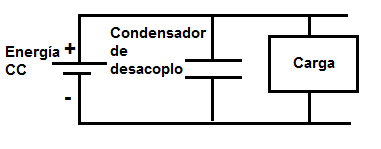
\includegraphics[width=8cm]{../Assets/condensador_desacople.png}

Analizando el sistema vemos que:
\[
	v_{in} - Ri(t) - \frac{q}{C} = 0
\]
\[
	V_c + V_p\sin(\omega t) = Ri(t) + \frac{1}{C}q
\]
Derivamos respecto a \(t\):
\[
	V_p\cos(\omega t)\omega = R\frac{di}{dt} + \frac{1}{C}i
\]
Resolviendo la ecuación diferencial tenemos que:
\[
	i(t) = i_0e^{\frac{-t}{RC}} + I_p\sin(\omega t)
\]
Si \(t \to \infty \Rightarrow i_0e^{\frac{-t}{RC}} \to 0\) \\
\(\Rightarrow v_{out} \sim V_p\sin(\omega t)\)

\subsection{Diagrama de fase} % Este nombre me lo invente yo, no se si esta bien puesto
% Esto no va en el orden de las diapositivas pero lo dimos justo al lado
Usamos que \(j=\sqrt{-1}\).
\[
	\begin{array}{ll}
		\text{En el tiempo:}                            & \text{En frecuencia:}                \\ \hline
		v(t)= V_p\cos(\omega t)                         & Re\{V_pe^{j\omega t}\}               \\
		i(t) = I_p\cos(\omega t + \phi)                 & Re\{I_pe^{j(\omega t + \phi)}\}      \\
		\frac{di}{dt} = -I_p\omega\sin(\omega t + \phi) & Re\{I_pj\omega e^j(\omega t +\phi)\}
	\end{array}
\]
\[
	V_pe^{j\omega t} = \frac{I_pj\omega}{C}e^j(\omega t +\phi) + RI_pe^{j(\omega t + \phi)}
\]
Operando se obtiene que:
\[
	\frac{v_{out}}{v_{in}} = \frac{1}{\sqrt{1 + (RC\omega)^2}}
\]


\chapter{Instrumentos analógicos}

Siguen vigentes porque son baratos y muy sensibles entonces se pueden construir instrumentos que miden con muy buena precision de forma barata.
Tambien son demandados por las insdustrias.

\section{Galvanómetro}

\subsection{Funcionanmiento}
Tenemos un iman permanente con una bobina movil. A traves de la bobina movil circula la corriente, lo que induce una fuerza por ley de Faraday y esto genera un par magnético que rota la aguja. \\
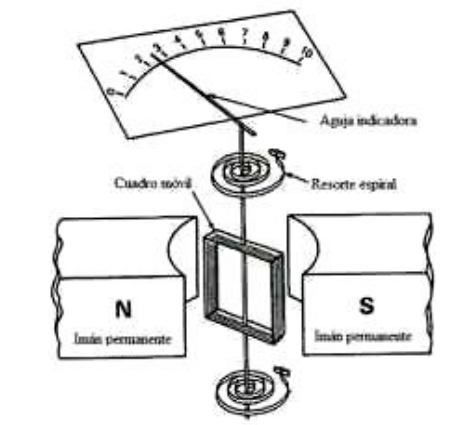
\includegraphics[width=8cm]{../Assets/galvanometro.png} \\
Cuando la bobina gira, arrastra la espira en cortocircuito que, por moverse en un campo magnético tendrá una f.e.m inducida y por tratarse de un circuito cerrado circula una intensidad inducida, que reacciona con el campo magnético generando un par que se opone al movimiento y que se llama AMORTIGUAMIENTO.

\subsection{Ecuacion diferencial de su movimiento}
\[
	J \frac{\partial^2{\theta}}{\partial{t^2}} = Gi - D \frac{\partial{\theta}}{\partial{t}} - k_r\theta
\]
Donde $J$ es el momento de inercia del rotor.

\subsection{Ley de respuesta de respuesta}
% Esto hay que chequearlo
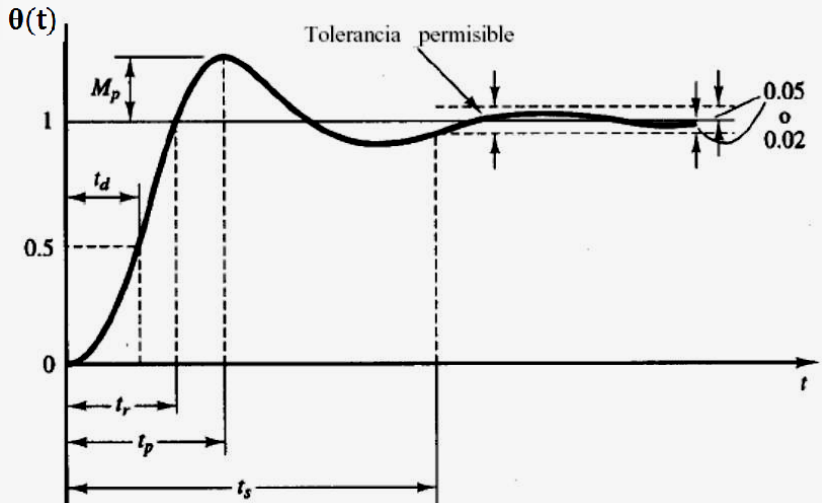
\includegraphics[width=8cm]{../Assets/instrumentos_analogicos_ley_de_respuesta.png}


\section{Amperímetro de DC}
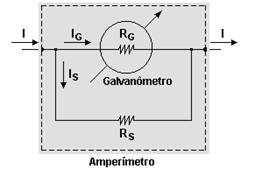
\includegraphics[width=8cm]{../Assets/amperimetro_galvanometro.jpg}


\section{Voltímetro de DC}
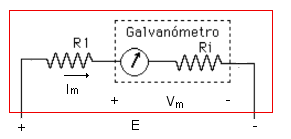
\includegraphics[width=8cm]{../Assets/voltimetro_galvanometro.png}

\section{Ohmetros}
\subsection{Ohmetros de derivación}

\subsection{Ohmetros serie}

\section{Amperimetro de AC}

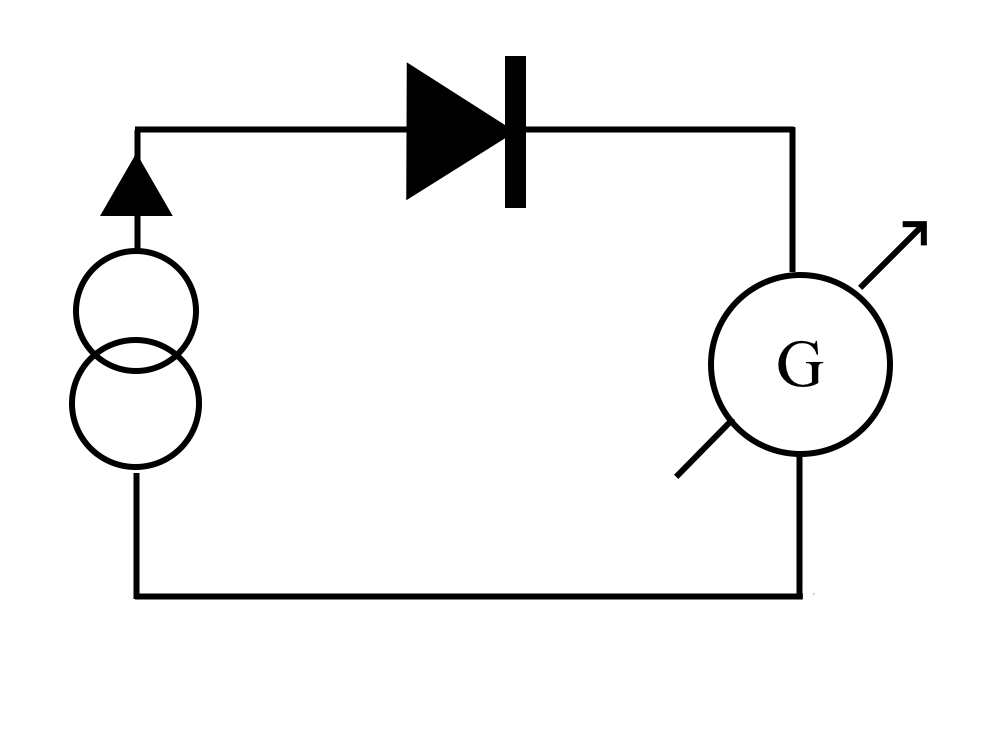
\includegraphics[width=8cm]{../Assets/amperimetro_galvanometro_ac.jpg}
\[
	\theta = k <i_g>
\]
\[
	<i_g> = \frac{1}{T}\int_{0}^{T}{i_g(t)dt} =
	\frac{1}{T}\int_{0}^{T/2}{\sqrt{2}I_{ef}\sin(\omega t)dt} =
	\frac{1}{T}\sqrt{2}I_{ef}\int_{0}^{T/2}{\sin(\omega t)dt}
\]
\[
	<i_g> = \frac{\sqrt{2}I_{ef}}{T}\left.\frac{-\cos(\omega t)}{\omega}\right|_0^{T/2} =
	\frac{\sqrt{2}I_{ef}}{\pi}
\]
\[
	\boxed{
		\theta = k \frac{\sqrt{2}}{\pi} I_{ef}
	}
\]
Vemos que si entra una onda sinusoidal, podemos colocar como salida simplemente la mimsa escala que en el amperimetro pero ajustada por la constante \(\frac{\sqrt 2}{\pi}\)

\chapter{Instrumentos digitales}
Estudiaremos los Digital MultiMeter (DMM). Estos son capaces de medir muchoas magnitudes.
Pueden medir tensión, intensidad de corriente, resitencia, temperatura, entre otras magnitudes.

Tiene 5 bloques que lo componen:
\begin{enumerate}
	\item Acondicionamiento de la señal de entrada
	\item Conversor Analógico Digital (CAD/DAC)
	\item Procesador digital
	\item Interfaz de entrada
	\item Interfaz de salida
\end{enumerate}

\section{Atenudor de tensión de CC}
Lo que hace es bajar la tensión \(V_e\).
Luego, amplifica la señal mediante un Amplificador Operacional (AO) para así obtener valores de tensión compatibles con el CAD.

\end{document}
